\begin{activity} \label{A:9.7.1} Let's investigate how we can interpret the derivative $\vr'(t)$. Let $\vr$ be the vector-valued function whose graph is shown in Figure \ref{F:9.7.VVF_tan_vector}, and let $h$ be a scalar that represents a small change in time. The vector $\vr(t)$ is the blue vector in Figure \ref{F:9.7.VVF_tan_vector} and $\vr(t+h)$ is the green vector.
\begin{figure}[ht]
\begin{center}
%\begin{minipage}{2.5in}
%\begin{center}
%\resizebox{!}{2.5in}{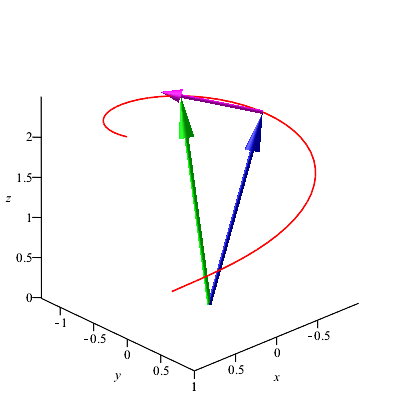
\includegraphics{9_7_VVFD_01}}
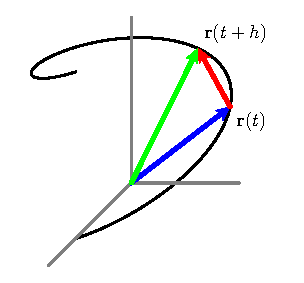
\includegraphics{fig_9_7_curve_1.eps}
\end{center}
\caption{A single difference quotient.}
\label{F:9.7.VVF_tan_vector}
%\end{minipage} \hspace{0.15in}
%\begin{minipage}{2.5in}
%\begin{center}
%\resizebox{!}{2.5in}{\animategraphics[controls]{4}{9_7_VVFD_}{01}{20}}
%\animategraphics[controls]{4}{figures/fig_9_7_animate_}{00}{07}
%\end{center}
%\caption{An animation of multiple difference quotients.}
%\label{F:9.7.VVF_tan_vector_animation}
%\end{minipage}
%\end{center}
\end{figure}
    \ba
    \item Is the quantity $\vr(t+h)-\vr(t)$ a vector or a scalar? Identify this object in Figure \ref{F:9.7.VVF_tan_vector}.

    \item Is $\frac{\vr(t+h)-\vr(t)}{h}$ a vector or a scalar? Sketch a representative vector $\frac{\vr(t+h)-\vr(t)}{h}$ with $h < 1$ in Figure \ref{F:9.7.VVF_tan_vector}.

    \item Think of $\vr(t)$ as providing the position of an object moving along the curve these vectors trace out.  What do you think that the vector $\frac{\vr(t+h)-\vr(t)}{h}$ measures? Why?  (Hint: You might think analogously about difference quotients such as $\frac{f(x+h) - f(x)}{h}$ or $\frac{s(t+h) - s(t)}{h}$ from calculus I.)

    \item Figure \ref{F:9.7.VVF_tan_vector_quotients} presents three snapshots of the vectors $\frac{\vr(t+h)-\vr(t)}{h}$ as we let $h \to 0$. Write 2-3 sentences to describe key attributes of the vector
        \[\ds \lim_{h \to 0} \frac{\vr(t+h)-\vr(t)}{h}.\]
         (Hint: Compare to limits such as $\lim_{h \to 0} \frac{f(x+h) - f(x)}{h}$ or $\lim_{h \to 0} \frac{s(t+h) - s(t)}{h}$ from calculus I, keeping in mind that in three dimensions there is no general concept of slope.)



    \ea
\begin{figure}[ht]
\begin{center}
%\begin{minipage}{2.5in}
%\begin{center}
%\resizebox{!}{2.5in}{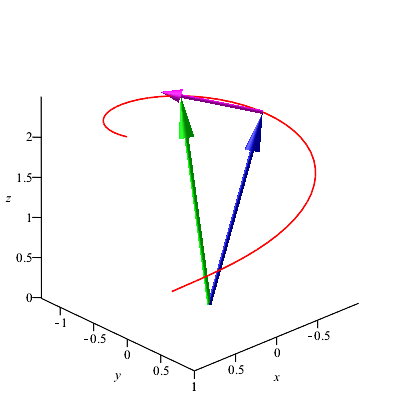
\includegraphics{9_7_VVFD_01}}
%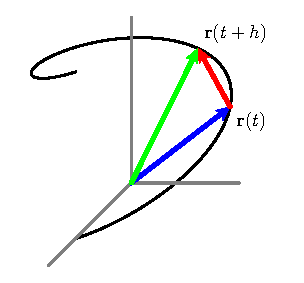
\includegraphics{fig_9_7_curve_1.eps}
%\end{center}
%\caption{A single difference quotient.}
%\label{F:9.7.VVF_tan_vector}
%\end{minipage} \hspace{0.15in}
%\begin{minipage}{2.5in}
%\begin{center}
%\resizebox{!}{2.5in}{\animategraphics[controls]{4}{9_7_VVFD_}{01}{20}}
%\animategraphics[controls]{4}{figures/fig_9_7_animate_}{00}{07}
\resizebox{!}{1.5in}{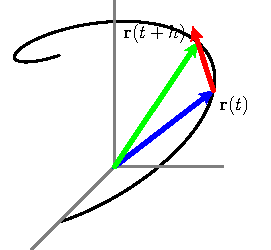
\includegraphics{fig_9_7_animate_02.pdf}} \hspace{0.25in} \resizebox{!}{1.5in}{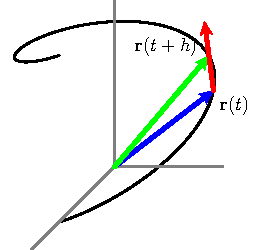
\includegraphics{fig_9_7_animate_04.pdf}} \hspace{0.25in} \resizebox{!}{1.5in}{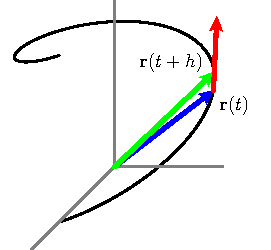
\includegraphics{fig_9_7_animate_06.pdf}} 
\end{center}
\caption{Snapshots of several difference quotients.}
\label{F:9.7.VVF_tan_vector_quotients}
%\label{F:9.7.VVF_tan_vector_animation}
%\end{minipage}
%\end{center}
\end{figure}
\end{activity}
\begin{smallhint}

\end{smallhint}
\begin{bighint}

\end{bighint}
\begin{activitySolution}
   \ba
    \item The quantity $\vr(t+h)-\vr(t)$ is a vector quantity, the vector from the terminal point of $\vr(t)$ to the terminal point of $\vr(t+h)$.

    \item The quantity $\frac{\vr(t+h)-\vr(t)}{h}$ is a vector quantity, it is a vector in the direction of $\vr(t+h)-\vr(t)$ that is $\frac{1}{h}$ times as long. 

    \item The vector $\vr(t+h)-\vr(t)$ represents a change in position of the object on the time interval $[t, t+h]$. When we multiply by $\frac{1}{h}$, we can consider this vector  $\frac{\vr(t+h)-\vr(t)}{h}$ as an average change of position, or the average velocity vector of the object on the interval $[t,t+h]$. 

    \item As $h \to 0$, the average velocity vectors $\frac{\vr(t+h)-\vr(t)}{h}$ approach the instantaneous velocity vector. The average velocity vector $\frac{\vr(t+h)-\vr(t)}{h}$ is a direction vector for the secant line to the curve that passes through the terminal points of $\vr(t)$ and $\vr(t+h)$. As we let $h \to 0$, these direction vectors approach a direction vector  
       \[\ds \lim_{h \to 0} \frac{\vr(t+h)-\vr(t)}{h}\]
of the tangent line to the curve at the terminal point of $\vr(t)$. 
    \ea

\end{activitySolution}
\aftera
